\section{Grundlagen}
%Im Grundlagenkapitel stellen Sie das Basiswissen für die weiteren Kapitel vor. 
%Hierzu können neben theoretischen Konzepten auch die historische Entwicklung 
%und aktuelle Forschungsvorhaben gehören. Idealerweise bedient man sich hier 
%mehrerer verschiedener Quellen, um die Ausführungen zu belegen.

%Nachfolgend werden einige Formalitäten der Arbeit dargestellt.

\subsection{Herausforderungen in Migrationsprojekten}
In \pcite{}{}{fivephases}  werden die folgenden wirtschaftlichen und 
technischen Faktoren identifiziert, die bei der Prüfung der Geeignetheit einer 
Anwendungs- oder Infrastrukturmigration berücksichtigt werden sollten.

\subsubsection{Wirtschaftliche Herausforderungen}
\begin{description}
	\item[Bereits getätigte IT-Investitionen:]
	Je größer das Unternehmen, das eine Anwendung in die Cloud migrieren 
will, desto größer sind die bereits getätigten Investitionen in die 
IT-Infrastruktur. Mit den Investitionen steigt in der Regel auch die 
Komplexität, was eine Migration erschwert.
	\item[Kosten:] Älteren Unternehmen fällt es aufgrund der langjährigen 
Erfahrung leicht die Kosten für die bestehende Softwarelösung abzuschätzen. 
Kosten, die zudem bereits genehmigt und eingeplant sind. Dem stehen die 
nutzungsbezogenen, bisher unbekannten Kosten einer Cloudlösung gegenüber. Diese 
Kosten sollten über eine Prognose der benötigten Rechen-, Speicher- und 
Transferkapazitäten, den Betriebs-, Lizenz- und Migrationskosten abgeschätzt 
werden, damit erhoffte Kosteneinsparungen auch tatsächlich realisiert werden 
können.
	\item[Datensicherheit:] Für den Unternehmenserfolg kritische Daten sind 
auf unternehmenseigenen Servern eventuell besser aufgehoben.
	\item[Rechtliche Restriktionen:] Das Unternehmen könnte rechtlichen 
Rahmenbedingungen ausgesetzt sein, die eine Migration in die Cloud ausschließen.
	\item[Zuteilung von Rechenleistungen:] Anwendungen, die kurzzeitig 
große Rechenleistungen benötigen und gut skalierbar sein sollen, lassen sich in 
der Cloud wahrscheinlich kostengünstiger betreiben als auf Servern die 
ganzjährig reserviert sind und sind damit geeignetere Kandidaten für eine 
Migration.
\end{description}

\subsubsection{Technische Herausforderungen}
\begin{description}
	\item[Bestehende Infrastruktur:] Mit der Infrastruktur, die sich im 
Laufe einer Migration ändert, ändert sich auch die Art, wie Anwendungen an 
Endnutzer ausgeliefert werden. Auch der Support wird möglicherweise nach der 
Migration nicht mehr über den IT-Support im Haus abgewickelt, sondern über den 
Cloud-Anbieter. 
	\item[Sicherheitsarchitektur:] Um die Daten im Cloud-Umfeld zu 
schützen, muss das bestehende Sicherheitskonzept an die Gegebenheiten der Cloud 
angepasst werden.
	\item[Komplexität:]
	Während einfache Anwendungen womöglich bereits in der Cloud angeboten 
werden, steigt mit der Komplexität auch der Planungs-, Implementierungs- 
und Testbedarf bei der Migration.
	\item[Netzwerk und Support:] Je mehr Daten in der Cloud liegen, desto 
höher ist die Abhängigkeit von einer funktionierenden Internetverbindung. Hier 
können zusätzliche Kosten für Verbindungen mit höheren Kapazitäten oder 
Verträge mit garantierten Reaktionszeiten im Störungsfall anfallen. Bei der 
Bewertung dieses Faktors schlage ich vor, die bereits vorhandene Abhängigkeit 
als Referenz zu nutzen. 
	\item[IT-Fähigkeiten:] Die Migration in die Cloud fordert dem IT-Team 
andere Fähigkeiten ab, als der lokale Betrieb und ist daher mit einer steileren 
Lernkurve verbunden. Sie geht außerdem regelmäßig mit einem Gefühl des 
Kontrollverlustes einher. 
	\item[Service Level Agreements (SLAs):] Geprüft werden sollte auch, ob 
Cloud-Anbieter SLAs bieten können, die zum unternehmerischen Bedarf 
hinsichtlich Verfügbarkeit, Vertraulichkeit und Integrität passen. Auch sollte 
geregelt sein, welche Verantwortlichkeiten der Anbieter trägt und welche 
Strafen bei Nichteinhaltung drohen.
\end{description}



\subsection{Methoden zur Anforderungsermittlung in Migrationsprojekten}
\subsection{Aktuelle und prognostizierte Ressourcennutzung}
\subsection{Auswahl des Migrationsziels in der Cloud}
\subsection{Kostenabschätzung der Cloud-Lösung}

\newpage
\subsection{Abbildungen}

\begin{figure}[h]
\begin{center}

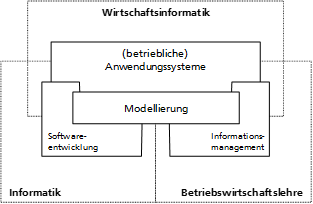
\includegraphics[width=10cm]{images/Abb2_3.png}
\caption{Einordnung der Wirtschaftsinformatik (angelehnt an Fink et al. 2001)}
\label{Abbildung2_3}
\end{center}
\end{figure}
Bitte achten Sie darauf, dass alle vorhandenen Abbildungen und Tabellen in einem inhaltlichen Zusammenhang mit dem Text stehen und Sie auf die entsprechende Abbildung (bspw. Abbildung 1) verweisen.
\subsection{Tabellen}
%hier Tabelle einfügen
\begin{table}[h]
\centering
\begin{tabular}{ccc}
\hline \textbf{Attribute} &\textbf{Typ}  & \textbf{1. Ausprägung (Beispiel)} \\ 
\hline Titel & \textit{STRING}& Aktiengesetz (AktG)  \\ 
Text& \textit{STRING} &  [Text des AktG]\\ 
Gültig von & \textit{DATE} & 01.01.2010 \\ 
Gültig bis & \textit{DATE} & - \\ 
Dok.-Besitzer & \textit{STRING} & Rechtsabteilung \\ 
Quelle & \textit{STRING}  & Deutsche Gesetze \\ 
Verplichtungsgrad & \textit{STRING} & verplichtend \\ 
\hline 
\end{tabular} 
\caption{Attribute der Anforderungsquellen im Metamodell}
\label{tab:tabelle 1}
\end{table}
\par\medskip

Tabelle 1 stellt eine beispielhafte Tabelle dar